\chapter{Vehicle Localization : The Guaranteed Estimation Problem} \label{ch:problem}
\section{Preliminaries}
The following standard notations are maintained in this paper.
\begin{itemize}
\item{$\mathcal{R}^n$ and $\mathcal{R}^{n \times m}$ denote the $n$ and $n \times m$ dimensional Euclidean space, respectively.}
\item{$I^n$ represents the $n$-identity matrix. If $n$ is missing, then appropriate dimension is assumed.}
\item{For a matrix $A$, $A^T$, $A^{-1}$, $A_{i}$ and $A^{j}$ denote its transpose, inverse, $i^{th}$ row, and $j^{th}$ column, respectively . $rs(A)$ is the row sum of $A$, and $det(A)$ the determinant.}
\item{$|.|$ is the absolute value and $||.||_{x}$ is the $x$-norm.}
\item{With a vector $a \in \mathcal{R}^n$, $diag(a)$ is a diagonal matrix of dimension $n$.}
\item{With a vector $a$, $n_a$ is its dimension.}
\item{For a real symmetric matrix, $P \in \mathcal{R}^{n \times n}, P \prec 0(P \succ 0)$ implies $P$ is a negative (positive) definite.}
\end{itemize}
\subsection{Zonotopes: Definitions and Properties}
The following definitions and properties are essential for this paper.
\begin{definition}\textbf{Interval} An interval $[a,b]$ is defined as the set $\{x : a \leq x \leq b\}$.
\begin{subdefinition}
The unitary interval, denoted by $\textbf{B}$, is [-1,1].
\end{subdefinition}
\begin{subdefinition}
A box( $( [a_1, b_1],..[a_n, b_n] )^T$ ) is an interval vector.
\end{subdefinition}
\begin{subdefinition}
An unitary box in $\mathcal{R}^n$ is denoted by $\textbf{B}^n$, and is a box with n unitary intervals.
\end{subdefinition}
\end{definition}
\begin{definition}
The Minkowski sum of two sets,$\mathcal{X}$ and $\mathcal{Y}$, is defined by: 
\begin{equation}
\mathcal{X} \bigoplus \mathcal{Y} = \{x+ y: x \in \mathcal{X}, y \in \mathcal{Y}\}
\end{equation}
\end{definition}
\begin{definition}
\textbf{Zonotope}:
An affine transformation of a hypercube, $\textbf{B}^m$ is called an $m$-ordered zonotope, denoted by $\mathcal{Z}\in \mathcal{R}^n$:\\
\begin{equation}
\mathcal{Z} = \langle p, H \rangle = \{p+ Hz: z \in \textbf{B}^m\}
\end{equation}
where $p \in \mathcal{R}^n$ is the center of $\mathcal{Z}$, and $H \in \mathcal{R}^{n \times m}$ is called the generator of $\mathcal{Z}$.
\end{definition}

\begin{lemma}
For two zonotopes, $\mathcal{Z}_1 = \langle p_1, H_1 \rangle$ and $\mathcal{Z}_2 = \langle p_2, H_2 \rangle$, the following equations hold:
\begin{equation}
\begin{split}
\mathcal{Z}_1 \bigoplus \mathcal{Z}_2 &= \langle p_1+p_2, [H_1 \quad H_2]\rangle \\
L\mathcal{Z}_1 &= \langle Lp_1, LH_1 \rangle 
\end{split}
\end{equation}
\end{lemma}
\begin{lemma} \cite{Althoff2010} \label{prop:overapprox}
A box of an $m$-zonotope , $\mathcal{Z} = \langle p, H \rangle \in \mathcal{R}^n$, is an $n$-interval vector, over-approximating the zonotope such that:
\begin{equation}
\lceil \mathcal{Z} \rceil = box(\mathcal{Z}) = [ p - \Delta H , p+ \Delta H], \quad \Delta H = \sum^{m}_{i=1} |H^i| 
\end{equation}
\end{lemma}
\begin{lemma}
\textbf{Zonotope Reduction} \cite{Alamo2005}, \cite{Combastel2003}: An $m$-zonotope ($\mathcal{Z} = \langle p, H \rangle \in \mathcal{R}^n$) can be reduced to an $s$-zonotope, s.t. $n < s < m$, by first sorting the columns of $H$ in decreasing order of Euclidean norm ($\hat{H}= [\hat{h}_1 ... \hat{h}_m]$, with $||\hat{h}_i||_2 \geq  ||\hat{h}_{i+1}||_2$). Then, let's split $\hat{H}$ into $\hat{H}_A$ (the first $s-n$ columns) and $\hat{H}_B$. Then the following inclusion is obtained:
\begin{equation}
\mathcal{Z} \subseteq p \bigoplus [\hat{H}_A \quad rs(\hat{H_B})]\textbf{B}^s \in \mathcal{R}^n
\end{equation}
It is denoted by $\mathcal{Z}_{\downarrow s}$ in this paper.
\end{lemma}

\begin{lemma}\label{prop:intersect} \cite{Alamo2005}
Given a zonotope $\mathcal{Z} = p \bigoplus H\textbf{B}^m \in \mathcal{R}^n$,
 a strip $\mathscr{S} = \{x \in \mathcal{R}^n : |cx-y| \leq \phi\}$, there exists a vector $\lambda \in \mathcal{R}^n$ such that a family of zonotopes parameterized by $\lambda$ contains the intersection of the zonotope and the strip s.t.:
\begin{equation}
\mathcal{Z} \cap \mathscr{S} \subseteq \mathcal{Z}(\lambda) =  p(\lambda) \bigoplus H(\lambda) \textbf{B}^{m+1}
\end{equation} 
with $p(\lambda) = p + \lambda(y - cp) \in \mathcal{R}^n$ \\
and $H(\lambda) = [(I - \lambda c)H \quad \phi \lambda]$ 

\end{lemma}
\begin{figure}[!h]
\label{fig:zonotope}
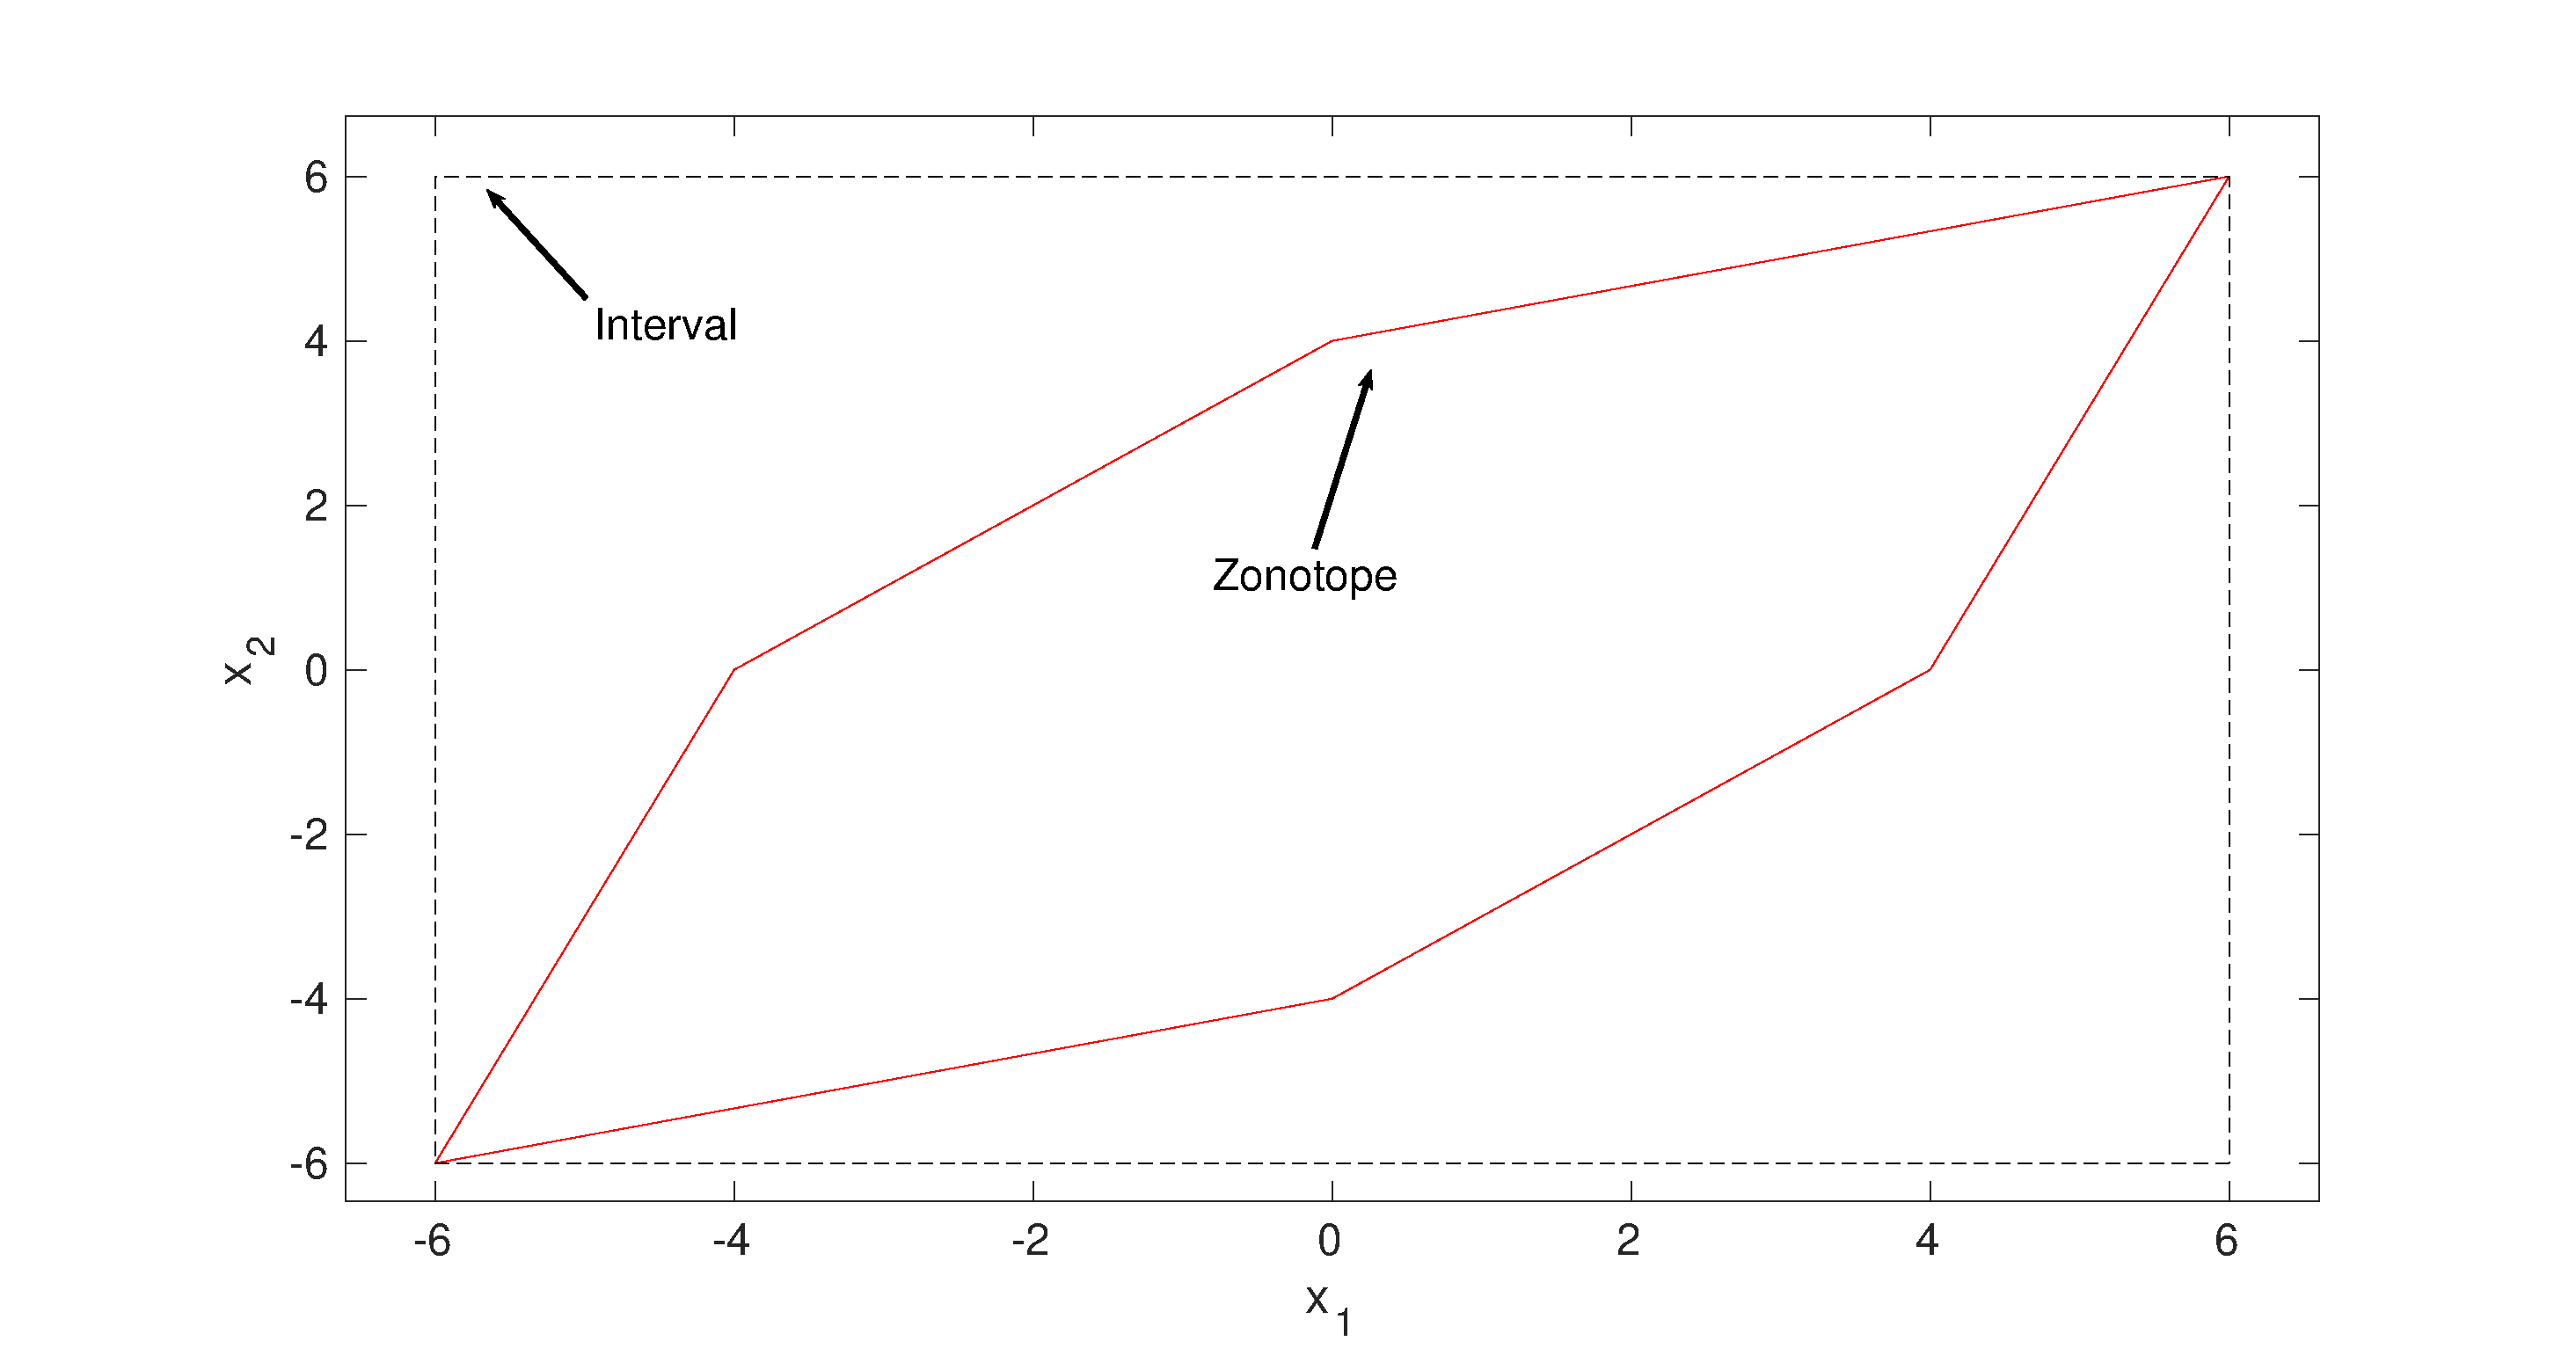
\includegraphics[scale=1, width=\linewidth]{figures/zonotope}
\caption{An illustration of a zonotope and its interval hull in 2-D}
\end{figure}
The construction, reduction, and interval calculation of zonotopes are implemented in the Matlab\textsuperscript{\tiny\textregistered} toolbox CORA (COntinuous Reachability Analyzer) \cite{Althoff2018}.
\section{Problem Formulation}
Let us denote the state of the vehicle to be tracked at time $k$ as $x_k$ and the measured state as $y_k$. Eq.~\eqref{formula:system} formuates a multi-output discrete-time linear system for the tracked vehicle, where $A, E \in \mathcal{R} ^{n_x \times n_x}$, $C \in \mathcal{R} ^{n_y \times n_x}$, and $F \in \mathcal{R} ^{n_y \times n_y}$ are matrices defined by the vehicle system model; $w_k$ and $v_k$ are process noise and measurement noise at time $k$, respectively. 
\begin{equation}
\label{formula:system}
\begin{split}
x_{k} &= Ax_{k-1} + Ew_k\\
y_k &= Cx_k + Fv_k
\end{split}
\end{equation}
Assuming $w_k$ and $v_k$ have known bounds ($\overline{w_k}$ and $\overline{v_k}$, respectively), we can define $\mathcal{W}$ and $\mathcal{V}$ such that $w_k \in \mathcal{W}$ and $v_k \in \mathcal{V}$ as \eqref{formula:wv}.
\begin{equation}
\label{formula:wv}
\mathcal{W} = \langle 0, H_w \rangle ,\quad \mathcal{V} = \langle 0, H_v \rangle
\end{equation}
The dimension of $x_k$ ($n_x$) varies across vehicle models; however, the measurement vector ($y_k$) is the measured position in the x and y-direction \eqref{formula:y}.  
\begin{equation}
\label{formula:y}
y =[ 
\begin{matrix}
s_x & s_y
\end{matrix}
]^T
\end{equation}
Given a vehicle model (discussed in the next section), the problem of set-based state estimation is to compute an outer bound of the state ($x_k$) containing all the possible values of the true state of the system consistent with the uncertain vehicle model and the measurements.
\section{Vehicle Model}
A major performance-influencing factor is to choose the right model for the tracked vehicle. Three linear systems are implemented in this paper to compare the state estimation algorithms. Although there exist highly precise vehicle models for ego vehicles, the simplest models are used here to represent the tracked vehicle, because complex vehicle models require parameters which are non-acquirable for tracked vehicles. In particular, physical dimensions, like wheelbase or side-slip, cannot be measured directly. Another reason is that adding some parameters, e.g. steering angle and yaw rate, makes the system non-linear and hence does not suit all the algorithms presented. Hence, the following models are investigated:
\begin{itemize}
\item \textbf{Constant Velocity (CV) Model}
\item \textbf{Constant Acceleration (CA) Model}
\item \textbf{Point-Mass (PM) Model}
\end{itemize}
\subsection{Constant Velocity Model}
The vehicle is assumed to travel in constant velocity \cite{Schubert2008}. The state of the system ($x_k$), state transition matrix ($A$), and the measurement matrix($C$) is shown in \eqref{formula:cvmodel}.
\begin{equation}
\label{formula:cvmodel}
\begin{split}
x &=
\left[\begin{matrix}
s_x & s_y & v_x & v_y
\end{matrix}\right]^{T}\\
A&= \left[\begin{matrix}
1 & 0 & \Delta T & 0\\
0 & 1 & 0 & \Delta T\\
0 & 0 & 1 & 0\\
0 & 0 & 0 & 1\\
\end{matrix}\right]\\
C&= \left[\begin{matrix}
1 & 0 & 0 & 0\\
0 & 1 & 0 & 0
\end{matrix}\right]
\end{split}
\end{equation}

\subsection{Constant Acceleration Model}
Although the constant velocity model is easy to implement, it is unrealistic to assume constant velocity. Acceleration model takes care of changing velocity and assumes constant acceleration \cite{Schubert2008}. Hence, the estimation errors for position and velocity are expected to be relatively smaller, when the velocity is constantly changing. The state of the system ($x_k$), the state transition matrix ($A$), and the measurement matrix($C$) are shown in \eqref{formula:camodel}.

\begin{equation}
\label{formula:camodel}
\begin{split}
x&= \left[\begin{matrix}
s_x & s_y & v_x & v_y & a_x & a_y
\end{matrix}\right]^{T}\\
A&= \left[\begin{matrix}
1 & 0 & \Delta T & 0 & \frac{1}{2}\Delta T^2 & 0\\
0 & 1 & 0 & \Delta T & 0 & \frac{1}{2}\Delta T^2 \\
0 & 0 & 1 & 0 & \Delta T & 0\\
0 & 0 & 0 & 1 & 0 & \Delta T\\
0 & 0 & 0 & 0 & 1 & 0\\
0 & 0 & 0 & 0 & 0 & 1
\end{matrix}\right] \\
C&= \left[\begin{matrix}
1 & 0 & 0 & 0 & 0 & 0\\
0 & 1 & 0 & 0 & 0 & 0
\end{matrix}\right]
\end{split}
\end{equation}

\subsection{Point-Mass Model}
It is trivial to note that vehicles might have varying acceleration, which is not satisfied in the previous models. This brings us to the point-mass model \cite{Althoff}, which is similar to the constant acceleration model, except that the acceleration here can strike up to a certain limit. This model treats the tracked vehicle as a point mass, ignoring wheel-base, slip-angle, etc. The state transition and measurement matrices are the same as the constant acceleration model (Eq.~\eqref{formula:camodel}). The acceleration bounds are set as $11.5 m/s^2$ \cite{Althoff} in both x and y-direction for this paper.

%\section{Domain Representation}
%The computation time of the algorithms largely varies due to the choice of shape to represent the set of state of the system. Zonotopes are gaining fame in the set-based state estimation techniques \cite{Le2013}, due to its control of wrapping effect and that the Minkowski sum of the zonotope results in zonotopes. The prediction step for the state estimation method can be simplified to basic matrix computation. The functionalities required in the correction step are implemented in the Matlab\textsuperscript{\tiny\textregistered} toolbox CORA (COntinuous Reachability Analyzer) \cite{Althoff2018}.
%
%Zonotopes are represented by a center, denoted by $p$ and generators, denoted by $H$. An m-zonotope in $\mathbb{R}^n$ can be defined as an affine transformation by $H$ of an m-dimensional hypercube in $\mathbb{R}^n$ centered at $p$. Minkowski sum, zonotope reduction, and the convex hull of zonotopes are required to be computed in the state estimation algorithms. The toolbox, CORA, is used to construct zonotopes and apply the computation for zonotopes in the algorithms. 
%\begin{figure}[!h]
%\label{fig:zonotope}
%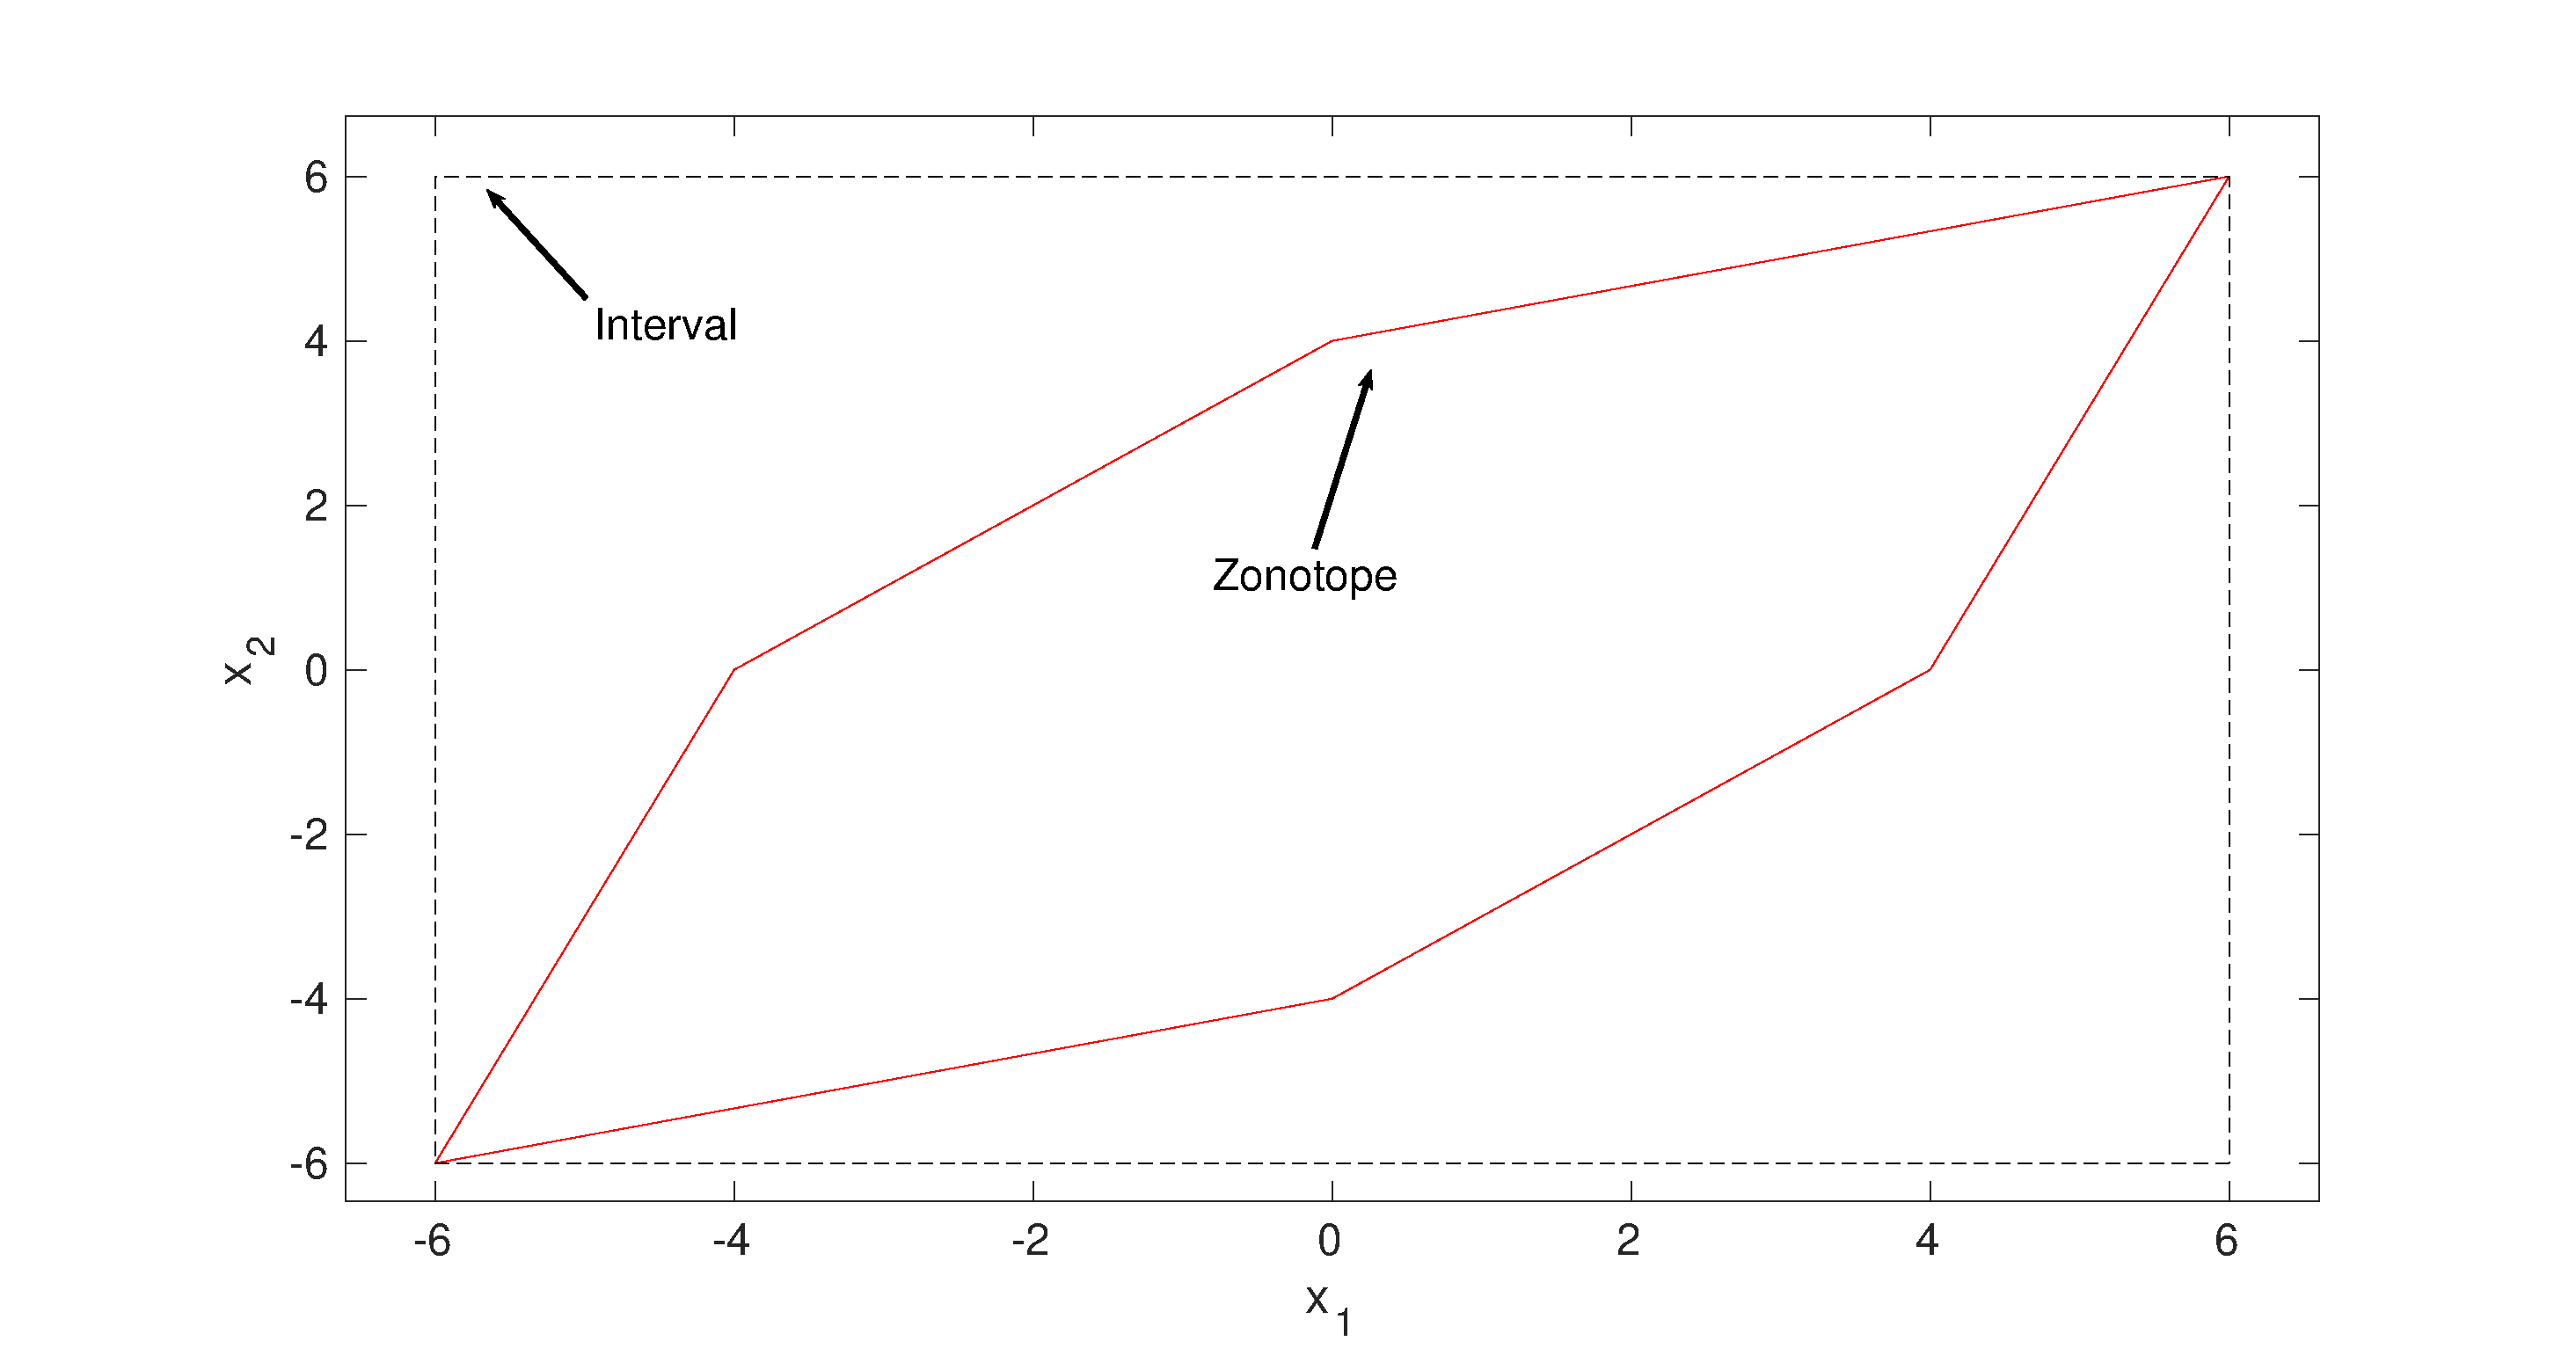
\includegraphics[scale=.25]{figures/zonotope}
%\caption{An illustration of a zonotope and its interval hull in 2-D}
%\end{figure}



